\subsection{Linux versioning scheme and development process}

\begin{frame}
  \frametitle{Linux versioning scheme}
  \begin{itemize}
  \item Until 2003, there was a new ``stable'' release branch of Linux every
        2 or 3 years (2.0, 2.2, 2.4). Development branches took 2-3
        years to be merged (too slow!).
  \item Since 2003, there is a new official release of Linux about every
	10 weeks:
  \begin{itemize}
	\item Versions \code{2.6} (Dec. 2003) to \code{2.6.39} (May 2011)
	\item Versions \code{3.0} (Jul. 2011) to \code{3.19} (Feb. 2015)
	\item Versions \code{4.0} (Apr. 2015) to \code{4.20} (Dec. 2018)
	\item Version \code{5.0} was released in Mar. 2019.
  \end{itemize}
  \item Features are added to the kernel in a progressive way. Since
        2003, kernel developers have managed to do so without having
        to introduce a massively incompatible development branch.
  \item For each release, there are bugfix and security updates called
    stable releases: 5.0.1, 5.0.2, etc.
  \end{itemize}
\end{frame}

\begin{frame}
  \frametitle{Linux development model}
  Using merge and bug fixing windows
  \begin{center}
    \includegraphics[width=\textwidth]{slides/sysdev-linux-intro-versioning/new-development-process.pdf}
  \end{center}
\end{frame}

\begin{frame}[fragile]
  \frametitle{Need for long term support (1)}
  \begin{itemize}
  \item Issue: bug and security fixes only released for most recent
    kernel versions.
  \item Solution: the last release of each year is made an LTS {\em (Long Term
     Support)} release, and is supposed to be supported (and receive bug
    and security fixes) for up to 6 years.
  \begin{columns}
  \column{0.6\textwidth}
  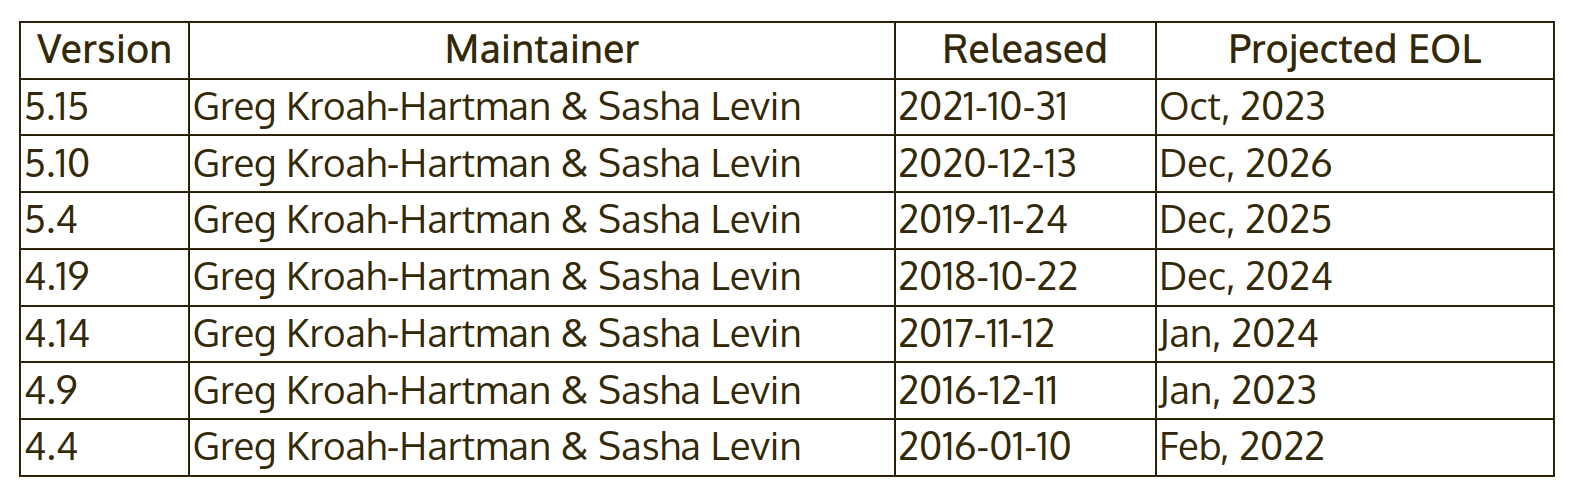
\includegraphics[width=\textwidth]{slides/sysdev-linux-intro-versioning/long-term-support-kernels.png}\\
  \column{0.4\textwidth}
  \scriptsize
   Captured on \url{https://kernel.org} in Nov. 2021, following the
   \href{https://www.kernel.org/category/releases.html}{\em Releases} link.
  \end{columns}
  \item Example at Google: starting from {\em Android O (2017)}, all new Android devices will
    have to run such an LTS kernel.
  \end{itemize}
\end{frame}

\begin{frame}[fragile]
  \frametitle{Need for long term support (2)}
  \begin{itemize}
  \item You could also get long term support from a commercial embedded
    Linux provider.
    \begin{itemize}
	\item Wind River Linux can be supported for up to 15 years.
	\item Ubuntu Core can be supported for up to 10 years.
    \end{itemize}
  \item {\em "If you are not using a supported distribution kernel, or a stable / longterm
    kernel, you have an insecure kernel"} - Greg KH, 2019\\
    Some vulnerabilities are fixed in stable without ever getting a CVE.
  \item The {\em Civil Infrastructure Platform} project is an industry /
    Linux Foundation effort to support selected LTS versions (starting
    with 4.4) much longer (> 10 years). See \url{https://bit.ly/2hy1QYC}.
  \end{itemize}
\end{frame}

\begin{frame}[fragile]
  \frametitle{What's new in each Linux release? (1)}
  The official list of changes for each Linux release is just a
  huge list of individual patches!
\Tiny
    \begin{verbatim}
commit aa6e52a35d388e730f4df0ec2ec48294590cc459
Author: Thomas Petazzoni <thomas.petazzoni@bootlin.com>
Date:   Wed Jul 13 11:29:17 2011 +0200

    at91: at91-ohci: support overcurrent notification

    Several USB power switches (AIC1526 or MIC2026) have a digital output
    that is used to notify that an overcurrent situation is taking
    place. This digital outputs are typically connected to GPIO inputs of
    the processor and can be used to be notified of these overcurrent
    situations.

    Therefore, we add a new overcurrent_pin[] array in the at91_usbh_data
    structure so that boards can tell the AT91 OHCI driver which pins are
    used for the overcurrent notification, and an overcurrent_supported
    boolean to tell the driver whether overcurrent is supported or not.

    The code has been largely borrowed from ohci-da8xx.c and
    ohci-s3c2410.c.

    Signed-off-by: Thomas Petazzoni <thomas.petazzoni@bootlin.com>
    Signed-off-by: Nicolas Ferre <nicolas.ferre@atmel.com>
\end{verbatim}
\normalsize
  Very difficult to find out the key changes and to get the
  global picture out of individual changes.
\end{frame}

\begin{frame}
  \frametitle{What's new in each Linux release? (2)}
  Fortunately, there are some useful resources available
  \begin{itemize}
    \item \url{https://kernelnewbies.org/LinuxChanges}\\
	In depth coverage of the new features in each kernel release
    \item \url{https://lwn.net/Kernel}\\
	Coverage of the features accepted in each merge window
  \end{itemize}
  \begin{center}
    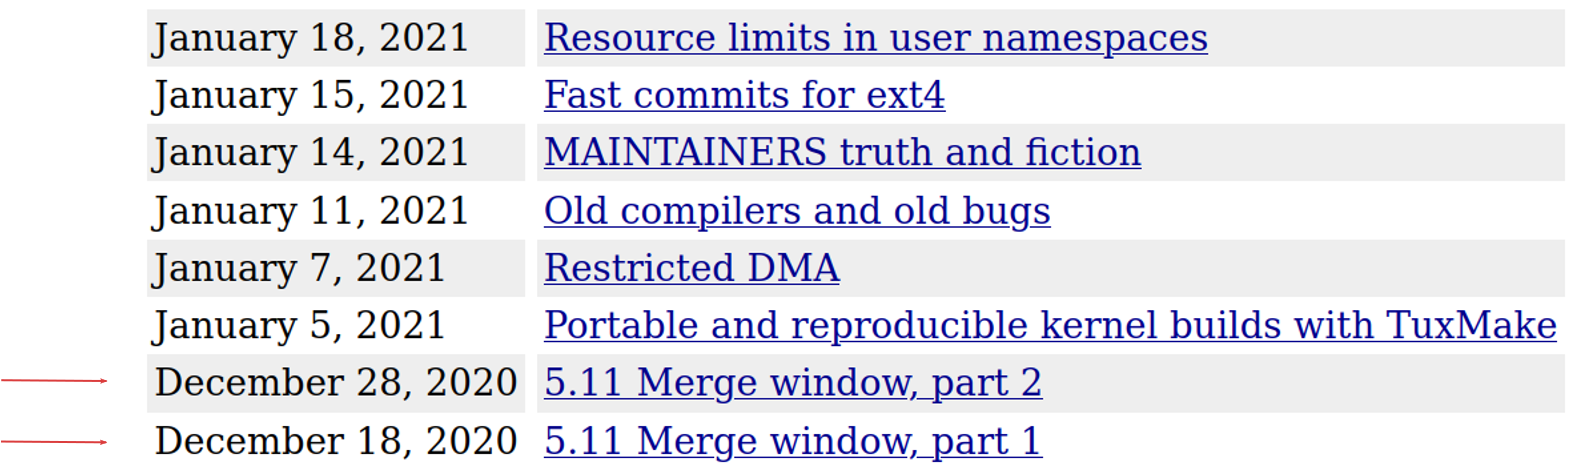
\includegraphics[width=0.8\textwidth]{slides/sysdev-linux-intro-versioning/lwn-kernel-articles.pdf}
  \end{center}
\end{frame}
